\chapter{Results and discussion}

\section{Effect of biocrust on soil aggregate stability (manuscript 1)}
\label{sec:BiocrustOnAggregateStability }

This study investigated the influence of biological soil crusts (biocrusts) on soil aggregate stability and their interplay with soil properties along a climatic gradient in the Chilean Coastal Range, spanning arid (PdA), semi-arid (SG), Mediterranean (LC), and humid (NA) conditions.

\subsection{Climate-induced changes in soil properties}
\label{sec:ClimateInducedSoil}

Soil properties varied significantly ($p < 0.05$) along the climate gradient (Figure \ref{fig:baseline_site}), reflecting the influence of increasing precipitation and decreasing temperature from north to south on weathering and soil development. Bulk density generally decreased from the drier northern sites (PdA: \SI{1.5}{\gram\per\cubic\centi\meter}, SG: \SI{1.6}{\gram\per\cubic\centi\meter}) to the humid south (NA: \SI{0.6}{\gram\per\cubic\centi\meter}). Conversely, soil organic carbon (SOC) content increased significantly along the gradient, from approximately \SI{0.3}{\percent} in PdA to \SI{12.5}{\percent} in NA, emphasizing the role of climate in organic matter accumulation. Total nitrogen (N\textsubscript{T}) followed a similar pattern, increasing from \SI{0.04}{\percent} in PdA to \SI{0.51}{\percent} in NA. However, the C/N ratio was highest at the climatic extremes (PdA: 33.9, NA: 24.5), potentially indicating nitrogen limitation in both the most arid and most humid environments, as suggested by Brust (2019). Soil pH decreased consistently and significantly along the gradient, from alkaline conditions in PdA (mean pH 7.7) to acidic conditions in NA (mean pH 4.4), likely due to increased leaching of base cations and higher biological acid production in wetter climates. Clay content also increased significantly from north (PdA: \SI{9.6}{\percent}) to south (NA: \SI{24.6}{\percent}).


\begin{sidewaysfigure}
    \centering
    % The \includegraphics command remains the same
    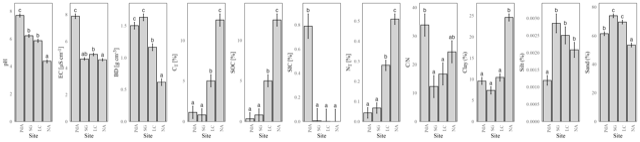
\includegraphics[width=1\textwidth]{img/baseline_by_site.png}
    % The caption remains the same
    \caption{Soil physical and chemical properties across the four study sites (PdA: Pan de Azúcar, SG: Santa Gracia, LC: La Campana, and NA: Nahuelbuta). Letter-based display accompanying soil properties with significant effect for site. Different letters indicate statistically significant differences ($p < 0.05$, Šidák correction).}
    % The label remains the same
    \label{fig:baseline_site}
\end{sidewaysfigure}

\FloatBarrier

\subsection{Biocrust-induced changes in soil properties}
\label{sec:BicorustInducedSoil}

Biocrust presence significantly ($p < 0.05$) influenced several soil properties (Figure \ref{fig:baseline_biocrust_interaction}a), often interacting with the climatic site (Figure \ref{fig:baseline_biocrust_interaction}b). A significant site $\times$ biocrust interaction was observed for bulk density, with biocrusts associated with a decrease in BD in arid PdA but an increase in Mediterranean LC. Biocrust presence significantly affected soil texture overall, associated with a slight decrease in clay and an increase in silt content when averaged across sites. However, the site $\times$ biocrust interaction was significant for clay, showing a notable increase under biocrusts specifically in PdA. Across all sites, biocrust presence led to a small but statistically significant decrease in soil pH, potentially reflecting localized acidification due to respiration \citep{Bachar2010}. C\textsubscript{T} and SOC contents were significantly lower under biocrusts when averaged across all sites. A significant site $\times$ biocrust interaction affected N\textsubscript{T}, showing significantly lower values under biocrusts only in the humid LC and NA sites. The C/N ratio was significantly lower under biocrusts overall, driven partly by changes in PdA. Electrical conductivity (EC) was extremely high in PdA compared to other sites, and the site $\times$ biocrust interaction showed a significant reduction in EC under biocrusts only in PdA.

% I will include it sideways for better visualization
\begin{sidewaysfigure}
    \centering
    % The \includegraphics command remains the same
    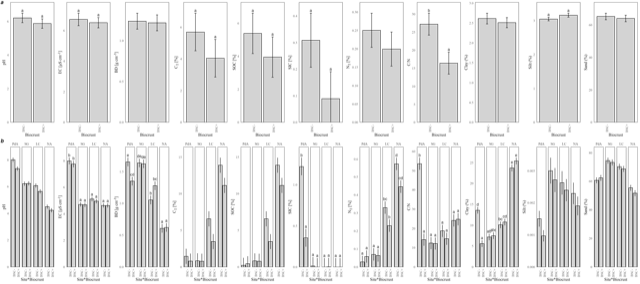
\includegraphics[width=1\textwidth]{img/baseline_by_biocrust_interaction.png}
    % The caption remains the same, clean up the p<0.05 part
    \caption{Biocrust (a) and interaction (b) effects on soil properties. Soil physical and chemical properties across for biocrust (BSC+ vs. BSC-) and the interaction with the site (PdA: Pan de Azúcar, SG: Santa Gracia, LC: La Campana, and NA: Nahuelbuta). Letter-based display accompanying soil properties with significant effect for site or site*biocrust. Different letters indicate statistically significant differences ($p < 0.05$, Šidák correction).} % Use math mode for p < 0.05
    % The label remains the same
    \label{fig:baseline_biocrust_interaction}
\end{sidewaysfigure} % *** End sidewaysfigure environment ***

\FloatBarrier

\subsection{Biocrust and climate interactions on aggregate stability}
\label{sec:BiocrusClimateInducedSoil}

Soil aggregate stability showed clear responses to both the climatic gradient and biocrust cover, particularly when assessed under wet conditions. Overall aggregate stability, indicated by the difference in geometric mean diameter ($\Delta$GMD), significantly increased (lower $\Delta$GMD indicates higher stability) along the climatic gradient from PdA (mean $\Delta$GMD \SI{1.86}{\milli\meter}) to NA (mean $\Delta$GMD \SI{0.83}{\milli\meter}), although SG showed higher stability (mean $\Delta$GMD \SI{1.2}{\milli\meter}) than LC (mean $\Delta$GMD \SI{1.4}{\milli\meter}). The water stability aggregate ratio (WSAR) confirmed this trend, with NA (mean WSAR 81.1\%) being significantly more stable than the other sites (mean WSAR 57.7\% - 73.4\%).

Biocrusts exerted a significant stabilizing effect, particularly on larger aggregates under wet sieving conditions. The presence of biocrusts significantly increased the proportion of water-stable aggregates $>$\SI{2}{\milli\meter} overall. Specifically, the interaction between site and biocrust was significant for wet aggregates in the \SIrange[range-phrase=--,range-units=single]{9.5}{30.0}{\milli\meter} range, showing a stabilizing effect (increase in proportion) in PdA, SG, and LC, but not in the humid NA site. This suggests a threshold effect, where the stabilizing role of biocrusts diminishes as vascular vegetation and associated stabilizing agents become more dominant under humid conditions. Correspondingly, biocrust presence significantly decreased the proportion of water-stable aggregates $<$\SI{2}{\milli\meter} (R\textsubscript{$<$\SI{2}{\milli\meter}}) overall (from mean 63.7\% without biocrusts to 57.5\% with biocrusts) (Figure \ref{fig:aggregate-stability}).

These findings highlight that biocrusts contribute to soil structure by binding particles and microaggregates, likely through mechanisms involving fungal hyphae, cyanobacterial filaments, and the production of extracellular polymeric substances \citep{Six2004,Totsche2018}. While biocrusts influenced bulk C and N contents, the lack of a direct correlation between these bulk changes and stability across all sites suggests that the specific composition and micro-spatial arrangement of organic binding agents within aggregates, rather than just total C or N, are critical for stability \citep{Wagner2007}. The results emphasize the crucial role of biocrusts as primary stabilizing agents in arid and semi-arid ecosystems \citep{BelnapBüdel2016}, with their influence gradually yielding to vascular plants and associated soil organic matter dynamics in more humid environments.

\begin{figure}[h!]
	\centering
	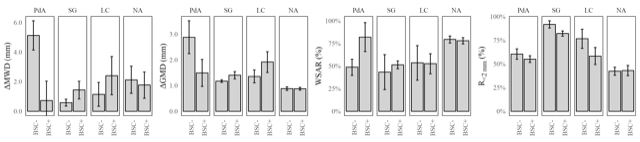
\includegraphics[width=1\textwidth]{img/aggregate stability indexes_se.png}
	\caption{Aggregate stability indexes for Pan de Azúcar (PdA), Santa Gracia (SG), La Campana (LC), and Nahuelbuta (NA) for biocrust (BSC+) and non-biocrust (BSC-) treatments displayes as mean and standard error. $\Delta$MWD: difference in mean weight diameter, $\Delta$GMD: difference in geometric mean diameter, WSAR: water stability aggregate ratio, R$_{<\SI{2}{\milli\meter}}$: ratio of aggregates less than \SI{2}{\milli\meter}.}
	\label{fig:aggregate-stability}
\end{figure}
\FloatBarrier

\section{Effect of biocrust on water flow, erosion and nutrient flow (manuscript 2)}
\label{sec:BiocrustOnFlows}

This study investigated the role of biological soil crusts (biocrusts) as climate-dependent regulators of erosion, water, and nutrient cycling using rainfall simulation experiments across a 910 km climate gradient in the Coastal Mountain Range of Chile. Four study sites represented coastal semi-arid (SG), inland semi-arid (QdT), Mediterranean (LC), and humid (NA) climates. These sites, characterized by comparable topography and granitic parent material, allowed for assessing biocrust influence under varying climatic conditions by comparing undisturbed soil monoliths with (+) and without (-) biocrust cover. We analyzed surface runoff, percolation flow, sediment transport, and associated carbon (C) and nitrogen (N) fluxes.

Soil properties varied across the climate gradient, reflecting differing weathering intensities and soil development stages relevant to hydrological and erosion responses. Notably, the inland semi-arid site (QdT) exhibited high biocrust cover despite lower water availability compared to the coastal SG site, likely due to protection from disturbance within a fenced area since 2011, fostering biocrust development \citep{Büdel2016}. Soil texture across sites was predominantly sandy loam, with clay content increasing southward, influencing water retention and infiltration pathways.

\subsection{Biocrust influence on water flow and sediment transport}
\label{sec:BiocrustOnWaterSesimentsFlows}

Biocrusts significantly modulated water flow and erosion dynamics, though their effects varied with climate and the specific pathway (runoff vs. percolation). Regarding runoff dynamics (Table \ref{tab:runoff_fluxes}), biocrusts delayed runoff initiation across all sites, with a mean delay of 97.7\%. This effect was particularly noticeable at the humid NA site, where dense bryophyte cover increased surface roughness and water storage \citep{Kidron2022}. Overall, biocrusts reduced total runoff volume by an average of 28.0\%, although this was site-specific, ranging from a 72.4\% reduction in NA to an unexpected 36.4\% increase in LC. Despite these impacts on surface flow, biocrusts did not measurably affect the time required for percolation to commence (Table \ref{tab:percolation_fluxes}). The reduction in runoff volume (Table \ref{tab:runoff_fluxes}) coupled with unchanged percolation timing (Table \ref{tab:percolation_fluxes}) indicated enhanced cumulative infiltration and saturated hydraulic conductivity in the presence of biocrusts compared to bare soil. In terms of erosion and sediment flux, biocrusts proved highly effective at reducing soil erosion via surface runoff, decreasing total sediment transport by an average of 69.9\% and sediment concentration in runoff by 60.9\% (Table \ref{tab:runoff_fluxes}). The most significant reduction occurred at the inland semi-arid QdT site, highlighting the protective role of biocrusts  \citep{RodriguezCaballero2018}. Conversely, sediment mobilization via percolation increased by 28.3\%, and sediment concentration in percolation rose by 58.3\% when biocrusts were present. This demonstrates a clear shift in sediment transport dynamics, moving from predominantly surface erosion on bare soil to increased subsurface transport under biocrust cover.

\begin{sidewaystable} % Using sidewaystable instead of table
    % \centering % Centering is often implicit/less relevant for full-page sideways tables
    \begin{threeparttable}
        \caption{Surface runoff fluxes on the study sites (SG: Santa Gracia, QdT: Quebrada de Talca, LC: La Campana, NA: Nahuelbuta) with (+) and without (-) biocrust (BSC) cover. Values correspond to mean $\pm$ standard deviation (SD) of five field replicates. Different letters indicate statistically significant different values based on Šidák correction post-hoc test results.}
        \label{tab:runoff_fluxes}

        % Define column widths/types. S columns align numbers. 'l' for text.
        % Determine table-format based on max digits before/after decimal, plus uncertainty.
        \begin{tabular}{@{} ll S[table-format=3.1(3.1)] l % Time
                             S[table-format=2.0(2.0)] l % Runoff
                             S[table-format=3.0(3.0)] l % Sediment
                             S[table-format=2.1(2.1)] l % Sed. Load
                       @{}}
            \toprule
            % --- Headers ---
            % Using \makecell for multi-line headers with units
            \multicolumn{2}{@{}l}{\textbf{Factor}} % Span first two columns for header alignment
            & \multicolumn{2}{c}{\makecell{\textbf{Time to start runoff}\tnote{a}\\ {[\si{\second}]}}}
            & \multicolumn{2}{c}{\makecell{\textbf{Runoff}\tnote{a}\\ {[\si{\liter\per\hour}]}}}
            & \multicolumn{2}{c}{\makecell{\textbf{Sediment in runoff}\tnote{a}\\ {[\si{\gram\per\meter\squared\per\hour}]}}}
            & \multicolumn{2}{c}{\makecell{\textbf{Sediment load of runoff}\tnote{a}\\ {[\si{\gram\per\liter\per\meter\squared}]}}} \\
            \cmidrule(lr){3-4} \cmidrule(lr){5-6} \cmidrule(lr){7-8} \cmidrule(lr){9-10} % Rules under spanned headers

            % --- Data Rows ---
            % Mean Site Effects
            Mean $\pm$ SD & SG   & 65.1 \pm 20.7  & (a) & 49 \pm 18  & (b) & 617 \pm 473 & (c) & 12.1 \pm 7.9  & (a) \\
                          & QdT  & 78.7 \pm 30.4  & (a) & 40 \pm 16  & (a) & 398 \pm 459 & (b) & 9.6 \pm 9.6   & (a) \\
                          & LC   & 83.5 \pm 56.0  & (a) & 39 \pm 22  & (a) & 241 \pm 293 & (b) & 7.3 \pm 8.8   & (a) \\
                          & NA   & 236.7 \pm 273.0& (b) & 44 \pm 43  & (a) & 28 \pm 44   & (a) & 3.0 \pm 14.0  & (a) \\
            \midrule
            % Mean Biocrust Effects
            Biocrust      & BSC+ & 154.0 \pm 211.5& (b) & 36 \pm 21  & (a) & 149 \pm 222 & (a) & 4.5 \pm 10.4  & (a) \\
                          & BSC- & 77.9 \pm 33.8  & (a) & 50 \pm 31  & (b) & 495 \pm 492 & (b) & 11.5 \pm 10.0 & (b) \\
            \midrule
            % Interaction Effects
            Site*Biocrust & SG BSC+ & 62.7 \pm 21.2 & (ab) & 44 \pm 16 & (ab) & 340 \pm 340 & (bc)  & 7.5 \pm 5.7  & (abc)  \\
                          & SG BSC- & 67.5 \pm 20.6 & (ab) & 54 \pm 18 & (ab) & 873 \pm 456 & (d)   & 16.7 \pm 7.1 & (de)   \\ \addlinespace
                          & QdT BSC+& 87.3 \pm 37.5 & (ab) & 38 \pm 15 & (ab) & 131 \pm 96  & (ab)  & 3.3 \pm 2.0  & (abd)  \\
                          & QdT BSC-& 70.1 \pm 18.7 & (ab) & 42 \pm 18 & (ab) & 665 \pm 524 & (cd)  & 15.8 \pm 10.2& (ce)   \\ \addlinespace
                          & LC BSC+ & 85.8 \pm 67.1 & (ab) & 45 \pm 20 & (ab) & 87 \pm 94   & (a)   & 2.1 \pm 1.9  & (a)    \\
                          & LC BSC- & 81.2 \pm 44.6 & (ab) & 33 \pm 23 & (ab) & 395 \pm 344 & (bc)  & 12.6 \pm 9.9 & (bcde) \\ \addlinespace
                          & NA BSC+ & 380.4 \pm 329.5& (b) & 19 \pm 23 & (a)  & 16 \pm 49   & (a)   & 5.2 \pm 19.9 & (abcde)\\
                          & NA BSC- & 93.0 \pm 40.2 & (a) & 69 \pm 45 & (b)  & 40 \pm 36   & (a)   & 0.9 \pm 1.2  & (abcde)\\
            \bottomrule
        \end{tabular}

        % --- Table Notes ---
        \begin{tablenotes}[para,flushleft] % para puts notes on one line if space, flushleft aligns note markers
           \item[a] Letter-based display accompanying surface runoff parameters. Different letters within a column section (Mean, Biocrust, or Site*Biocrust interaction) indicate statistically significant differences ($p < 0.05$, Šidák correction).
        \end{tablenotes}

    \end{threeparttable}
\end{sidewaystable} % *** End the sidewaystable environment ***


\begin{sidewaystable} % Using sidewaystable for landscape orientation
    \begin{threeparttable}
        \caption{Percolating water fluxes on the study sites (SG: Santa Gracia, QdT: Quebrada de Talca, LC: La Campana, NA: Nahuelbuta) with (+) and without (-) biocrust (BSC) cover. Values correspond to mean $\pm$ standard deviation (SD) of five field replicates. Different letters indicate statistically significant different values based on Šidák correction post-hoc test results.}
        \label{tab:percolation_fluxes} % Unique label for this table

        % Use tabular* to fill the linewidth.
        % Column structure MUST match Table 2: ll Sl Sl Sl Sl
        % Add 'l' columns even where no letters exist in Table 3.
        \begin{tabular*}{\linewidth}{@{\extracolsep{\fill}} % Distribute extra space
                             ll % Factor Column 1 & 2 (left aligned)
                             @{\extracolsep{\fill}} % Space after Factor columns
                             S[table-format=3.0(3.1)] l % Time Column 3 (S) + EMPTY Letter Column 4 (l)
                             @{\extracolsep{\fill}} % Space after Time group
                             S[table-format=2.1(2.0)] l % Percolation Column 5 (S) + Letter Column 6 (l)
                             @{\extracolsep{\fill}} % Space after Percolation group
                             S[table-format=2.0(2.0)] l % Sediments Column 7 (S) + Letter Column 8 (l)
                             @{\extracolsep{\fill}} % Space after Sediments group
                             S[table-format=1.1(2.1)] l % Sed. Load Column 9 (S) + EMPTY Letter Column 10 (l)
                             @{} % No padding at the end
                             }
            \toprule
            % --- Headers ---
            % Span 2 columns (S+l) for EACH parameter header for consistent layout
            \multicolumn{2}{@{}l}{\textbf{Factor}}
            & \multicolumn{2}{c}{\makecell{\textbf{Time to start}\\\textbf{percolation flow}\\ {[\si{\second}]}}}
            & \multicolumn{2}{c}{\makecell{\textbf{Percolation}\tnote{a}\\ {[\si{\liter\per\hour}]}}}
            & \multicolumn{2}{c}{\makecell{\textbf{Sediments in}\\\textbf{percolation flow}\tnote{a}\\ {[\si{\gram\per\meter\squared\per\hour}]}}}
            & \multicolumn{2}{c}{\makecell{\textbf{Sediment load in}\\\textbf{percolation}\\ {[\si{\gram\per\liter\per\meter\squared}]}}} \\
            % cmidrules span 2 cols each, matching headers
             \cmidrule(lr){3-4} \cmidrule(lr){5-6} \cmidrule(lr){7-8} \cmidrule(lr){9-10}

            % --- Data Rows ---
            Mean $\pm$ SD & SG   & \num{223 \pm 190}   &     & \num{18.0 \pm 14}  & (a) & \num{19 \pm 34} &     & \num{4.2 \pm 19.7} &   \\
                          & QdT  & \num{175.0 \pm 94.5}&     & \num{22.8 \pm 15}  & (a) & \num{7 \pm 10}  &     & \num{0.2 \pm 0.3}  &   \\
                          & LC   & \num{234 \pm 183}   &     & \num{22.4 \pm 13}  & (a) & \num{13 \pm 15} &     & \num{0.5 \pm 0.5}  &   \\
                          & NA   & \num{145 \pm 169}   &     & \num{65.0 \pm 39}  & (b) & \num{23 \pm 25} &     & \num{0.4 \pm 0.4}  &   \\
            \midrule
            Biocrust      & BSC+ & \num{171 \pm 133}   &     & \num{42.6 \pm 34}  & (b) & \num{19 \pm 22} & (b) & \num{0.5 \pm 0.5}  &   \\
                          & BSC- & \num{218 \pm 190}   &     & \num{21.5 \pm 21}  & (a) & \num{12 \pm 24} & (a) & \num{2.1 \pm 13.7} &   \\
            \midrule
            Site*Biocrust & SG BSC+  & \num{202 \pm 103}   &     & \num{24.8 \pm 15}  & (ab) & \num{19 \pm 18} &     & \num{0.7 \pm 0.5}  &   \\
                          & SG BSC-  & \num{244 \pm 251}   &     & \num{11.1 \pm 10}  & (a)  & \num{18 \pm 46} &     & \num{7.5 \pm 27.5} &   \\ \addlinespace
                          & QdT BSC+ & \num{148.0 \pm 63.9}&     & \num{30.5 \pm 13}  & (b)  & \num{9 \pm 13}  &     & \num{0.3 \pm 0.3}  &   \\
                          & QdT BSC-& \num{202 \pm 113}   &     & \num{15.1 \pm 13}  & (ab) & \num{5 \pm 6}   &     & \num{0.2 \pm 0.2}  &   \\ \addlinespace
                          & LC BSC+  & \num{226 \pm 223}   &     & \num{23.5 \pm 14}  & (ab) & \num{17 \pm 19} &     & \num{0.6 \pm 0.5}  &   \\
                          & LC BSC-  & \num{241 \pm 139}   &     & \num{21.3 \pm 14}  & (ab) & \num{9 \pm 9}   &     & \num{0.4 \pm 0.3}  &   \\ \addlinespace
                          & NA BSC+  & \num{107.0 \pm 35.6}&     & \num{91.5 \pm 28}  & (c)  & \num{30 \pm 32} &     & \num{0.4 \pm 0.4}  &   \\
                          & NA BSC-  & \num{183 \pm 234}   &     & \num{38.5 \pm 30}  & (b)  & \num{16 \pm 15} &     & \num{0.4 \pm 0.3}  &   \\

            \bottomrule
        \end{tabular*} % End tabular*

        % --- Table Notes ---
        \begin{tablenotes}[para,flushleft]
           \item[a] Letter-based display accompanying parameters where shown. Different letters within a column section (Mean, Biocrust, or Site*Biocrust interaction) indicate statistically significant differences ($p < 0.05$, Šidák correction).
        \end{tablenotes}

    \end{threeparttable}
\end{sidewaystable} % End the sidewaystable environment

\FloatBarrier

\FloatBarrier

\subsection{Biocrust modulation of carbon and nitrogen fluxes}
\label{sec:BiocrustOnNutrientFlows}

Biocrusts significantly altered the transport pathways and amounts of C and N in both sediment-bound and dissolved forms, with effects dependent on climate and site conditions (Figure \ref{fig:nutrient-flow}). For carbon fluxes, sediment-associated C loss via runoff generally increased with climatic humidity. Biocrusts significantly reduced this sediment C loss, by up to a factor of four compared to bare soil. In percolation flow, biocrusts also reduced the C content in mobilized sediments, an effect most pronounced in drier climates where reductions reached 20-40\%. Furthermore, biocrusts consistently increased dissolved organic carbon (DOC) concentrations in runoff across all sites, suggesting an alteration of C cycling pathways towards leaching rather than just physical erosion \citep{Baumert2021}. Similar patterns, though moderated by site*biocrust interactions, were observed for DOC transported via percolation. Regarding nitrogen fluxes, sediment-associated N loss via runoff also increased with humidity. The biocrust effect on this sediment N was strongly site-specific, causing an increase in SG but a decrease in NA, and explaining 48.8\% of the observed variability. Dissolved organic nitrogen (DON) fluxes in runoff showed trends analogous to DOC, generally increasing with biocrust presence, especially in northern sites like SG (increasing from 1.3$\pm$1.0 ppm in BSC- to 2.2$\pm$2.0 ppm in BSC+). However, a contrasting effect was observed at the humid NA site, where biocrusts decreased DON in runoff (from 0.6$\pm$0.7 ppm in BSC- to 0.3$\pm$0.8 ppm in BSC+), potentially indicating enhanced N immobilization or uptake in this N-richer ecosystem. DON fluxes transported via percolation followed similar site-dependent trends influenced by biocrust interactions.

\begin{figure}[h!]
	\centering
	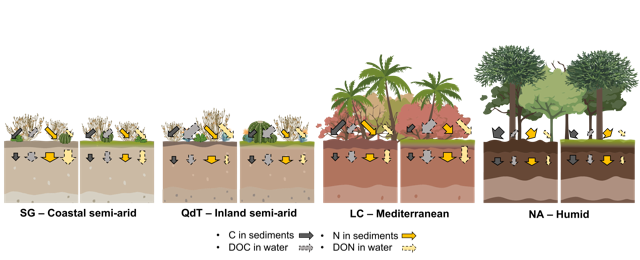
\includegraphics[width=1\textwidth]{img/nutrient-flow-diagram.png}
	\caption{Representation of total carbon in sediments and DOC in water fluxes for the four study sites. The diagrams at the right side with slightly green surface represents the BSC+ treatments and the one at the left the BSC-. Grey-filled arrows correspond to C fluxes, and yellowish arrows to N. At the same time, arrows with solid borders correspond to the flow attached to the sediments, and dashed arrows dissolved in water. Each type of arrow is proportional inside each group in width to the concentration of nutrients and in length to the mass of it.}
	\label{fig:nutrient-flow}
\end{figure}

\FloatBarrier

Overall, biocrusts play a crucial, climate-dependent role in regulating water flow, significantly reducing surface runoff erosion, but potentially increasing subsurface sediment transport. They profoundly influence C and N cycling, generally reducing C losses via runoff while altering dissolved nutrient pathways, with specific effects on N mobilization varying strongly between arid and humid environments.

\section{Microbial, plant and moisture controls on soil structure and functionality (Manuscripts 3, 4 and 5)}
\label{sec:MicrobesPlantsMoistureStructure}

Beyond the direct impacts of biological soil crusts (BSCs) and the broad climatic gradient, further investigations using subsets of the study sites (primarily arid Pan de Azúcar (PdA) and semi-arid Santa Gracia (SG), but also including mediterranean La Campana (LC) and humid Nahuelbuta (NA) in Manuscript 4) provided deeper insights into the roles of the indigenous microbial community, plant roots, and moisture dynamics in shaping soil aggregation, organic matter turnover, and nutrient cycling. These studies employed controlled laboratory incubations simulating specific scenarios: a shift to humid conditions for arid/semi-arid soils (Manuscript 3), repeated wetting-drying (W-D) versus constant moisture (CM) regimes across the climate gradient (Manuscript 4), and the natural transition from a living rhizosphere to a decomposing detritusphere in semi-arid soil (Manuscript 5).

A central finding emerging from these experiments is that the impact of microbial activity on soil aggregation and related properties is highly dependent on the origin of the soil and the prevailing environmental conditions. This was clearly demonstrated in the moisture regime experiment (Manuscript 4), where the responses of native, microbially active soils to repeated wetting-drying (W-D) cycles were compared against sterilized controls across the climate gradient. Principal Component Analysis visually distinguished the trajectories of native versus sterile soils under W-D stress, directly highlighting the significant contribution of microbial activity to changes in soil edaphic properties (Figure \ref{fig:PCA-microbes}). Crucially, the nature of this microbial influence differed markedly between climate zones. In arid soils, the microbially-influenced samples were primarily characterized by changes in aggregate C/N ratios, suggesting accelerated turnover of labile organic matter (OM) fueled by the Birch effect (Figure \ref{fig:PCA-microbes}A). In contrast, microbially-influenced semi-arid and mediterranean soils under W-D were distinguished from controls mainly by shifts in aggregate size distribution, particularly an increase in microaggregates (MIC) relative to macroaggregates (MAC) (Figure \ref{fig:PCA-microbes}B-C). This direct comparison underscores that while microbes actively mediate soil structural changes during moisture fluctuations, the specific mechanisms and outcomes (OM turnover vs. aggregate reorganization) are strongly dictated by the climate legacy imprinted on the soil and its microbial community.

\begin{figure}[h!]
	\centering
	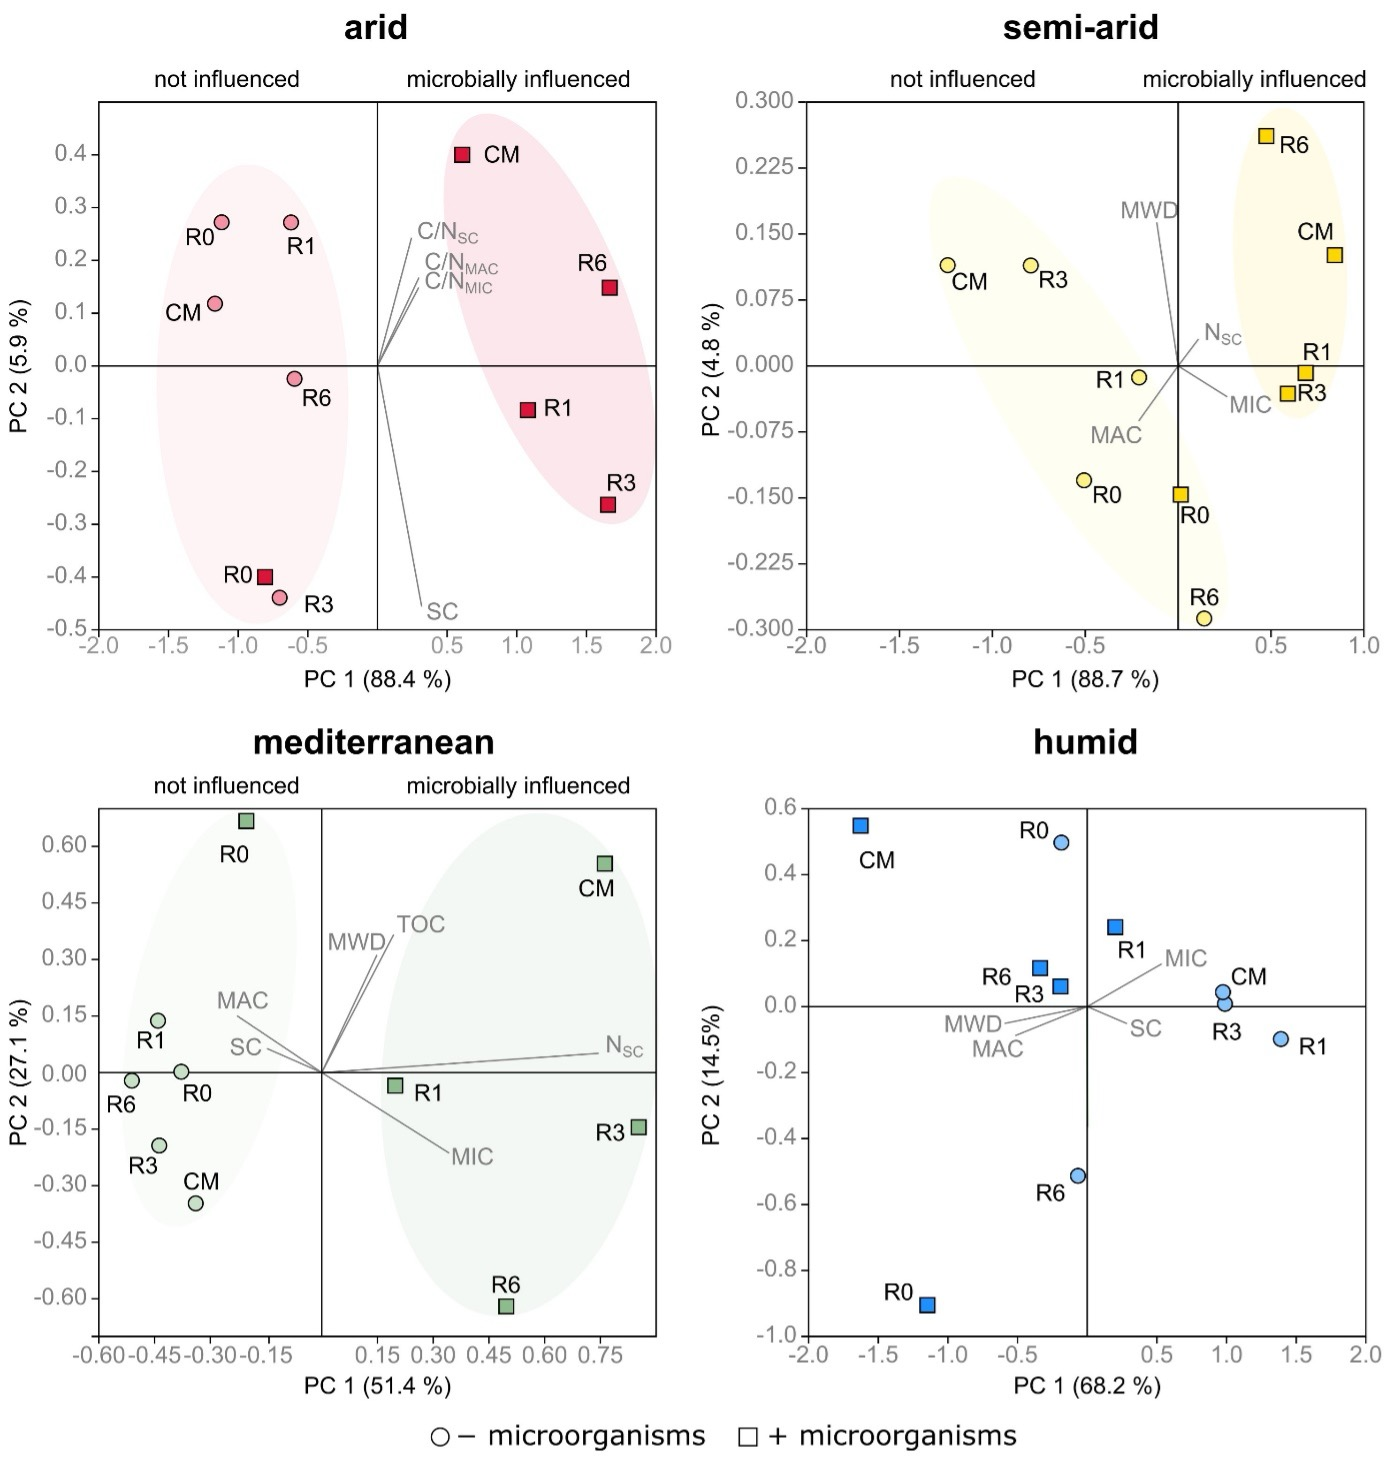
\includegraphics[width=1\textwidth]{img/PCA-microbes-structure.jpg}
	\caption{Principal Component Analyses of soil properties in native soils (squares) and sterilized soils (circles) including significant soil properties. A) arid, B) semi-arid, C) mediterranean and D) humid site. Microbial influence is indicated by sample separation along the x-axis.}
	\label{fig:PCA-microbes}
\end{figure}

\FloatBarrier

Further results support this picture of context-dependent microbial influence and climate legacy effects. The observed increase in aggregate C/N ratios in microbially active arid soils (Figure \ref{fig:bacterial-abundance}A) aligns with findings of stimulated microbial abundance under W-D but also a net breakdown of MAC and only a slight decrease in overall aggregate stability (MWD) (Manuscript 4), consistent with rapid consumption of labile OM released from decomposing larger aggregates. The microaggregate formation observed in microbially influenced semi-arid and mediterranean soils (Figure \ref{fig:PCA-microbes}B-C) corresponds with outcomes where overall stability either slightly decreased (semi-arid) or increased (mediterranean) (Manuscript 4), suggesting different stabilization pathways potentially involving OM redistribution or transformation.

\begin{figure}[h!]
	\centering
	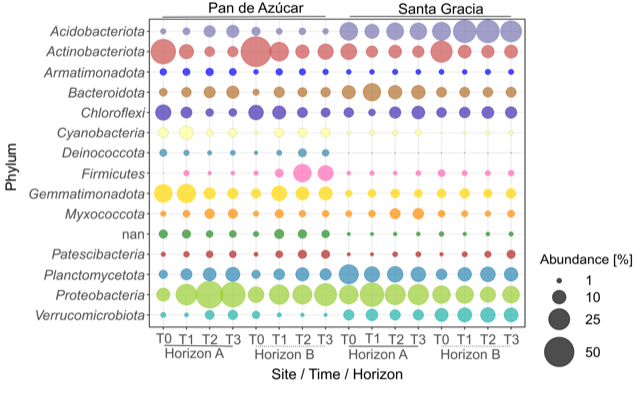
\includegraphics[width=1\textwidth]{img/bacterial-abundance.png}
	\caption{Relative abundance of top 15 bacterial phyla for Pan de Azúcar and Santa Gracia and the different time points. Time is represented as T0 (original), T1 (2 weeks), T2 (12 weeks) and T3 (16 weeks). Each bubble is the mean of the different treatments (in situ, BSCs and plants) and technical triplicates.}
	\label{fig:bacterial-abundance}
\end{figure}

\FloatBarrier

The importance of climate legacy was also evident in the differential resilience of microbial communities themselves. The arid PdA community, adapted to stable hyperaridity, showed significant structural changes and diversity loss under simulated humid conditions (Manuscript 3), while the semi-arid SG community, from a more variable climate, demonstrated greater stability (Figure \ref{fig:bacterial-abundance}), mirroring the patterns observed in the PCA analysis (Figure \ref{fig:PCA-microbes}).

Beyond the intrinsic microbial community and moisture effects, the powerful role of plants was confirmed (Manuscript 5). Living roots acted as potent drivers of macroaggregation in both topsoil and subsoil of semi-arid origin. However, a distinct root legacy effect was apparent, as this enhanced aggregation only persisted after plant death in the topsoil, indicating a requirement for continuous C input or greater inherent stability factors in the subsoil. This transition from rhizosphere to detritusphere also drove a microbial succession from fungal to Gram-positive bacterial dominance and altered OM protection mechanisms, notably increasing occluded POM in the topsoil detritusphere.
